\chapter{Architettura Funzionale del Sistema}
\label{chap:systemdesign}
\section{Funzionamento dell'Applicazione}
\subsection{Scenario}
Lo scopo di quest'applicazione è quello di \textit{velocizzare l'accesso i servizi}. Senza questo \textit{primo requisito}, l'applicazione non troverebbe posto nel mondo enterprise. Per questo motivo, l'interfaccia utente risulta semplice, e comprende poche funzionalità. 
\paragraph{L'utente} per accedere ai servizi deve registrarsi al sistema fornendo i propri dati personali (che potranno essere modificati in qualsiasi momento), scegliendo un'email e una password per le future autenticazioni. Anche senza essere registrato può cercare una struttura tra quelle presenti e scegliere un servizio che questa eroga. 
\paragraph{I servizi} possono essere diversi: analisi, esami, visite mediche, qualsiasi servizio che preveda un'attesa del cliente potrebbe essere inserito da una struttura sanitaria. Selezionando un servizio, all'utente viene mostrato il relativo calendario di disponibilità, in termini di giorni e fasce orarie. 
\paragraph{La prenotazione} avviene una volta selezionato un orario (corrispondente a uno \emph{slot}) e confermata l'intenzione di volerlo riservare. Per fare quest'operazione è necessario che l'utente sia autenticato al sistema. Prima di confermare la prenotazione di uno slot, l'utente può scegliere se inserire i dati (almeno uno tra nome e cognome, email o telefono) di un altro utente, anche non iscritto al sistema, per cui prenotare il servizio. Scegliendo questa opzione il destinatario sarà informato mediante delle notifiche sui futuri eventi relativi allo stato della sua prenotazione. A questo punto all'utente viene fornito un ``biglietto virtuale''.
\paragraph{Il biglietto} consiste in una numerazione. Questa numerazione corrisponde al numero che verrà chiamato allo sportello (si pensi ad un biglietto virtuale staccato al momento della prenotazione). Ciascun servizio è identificato da una lettera dell’alfabeto (A, B, C, \dots) mentre ciascun numero identifica il cliente in coda (1, 2, 3, \dots). In questo modo la numerazione B12, ad esempio, fa riferimento al cliente numero 12 di un servizio, C13 ad un altro cliente di un altro servizio. L’idea è che chi ha prenotato acceda alla struttura nel momento esatto in cui viene erogato il servizio, evitando coda e assembramenti.
\paragraph{La struttura}, così come l’utente, deve avere informazione di questo biglietto virtuale e questo avviene attraverso un \textsl{software} installato in loco che prende il nome di \textbf{mru}.
\paragraph{L'MRU} è un software che disponde di un'interfaccia web per gli operatori e per i totem che vengono utilizzati. Tutte le notti l'MRU interroga Zerocoda richiedendo le prenotazioni per la giornata odierna. Se ci sono le scarica, in questo modo anche gli operatori hanno informazione delle prenotazioni.

\subsection{Use Case Diagram}
\begin{figure}[H]
    \centering
    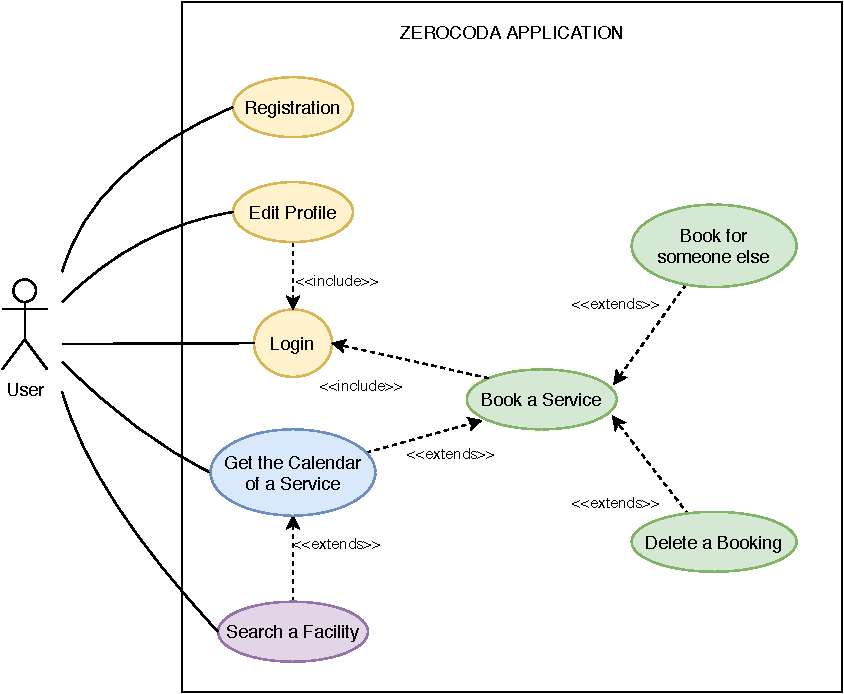
\includegraphics[width=0.94\textwidth]{images/02_2_zerocoda_usecase.pdf}
    \caption{Zerocoda Use Case Diagram}
    \label{fig:zerocodausecase}
\end{figure}
In figura [\ref{fig:zerocodausecase}] è presentato il diagramma dei casi d'uso di un utente generico di Zerocoda. I diversi colori utilizzati per le operazioni che può fare rappresentano la \textit{divisione in servizi} scelta per la fase di implementazione delle REST Api.

\subsection{I diversi Enti Zerocoda}
Sull'applicazione Zerocoda è possibile prenotare i servizi erogati da diversi enti. Alcuni di questi, tuttavia, non sono presenti sul sito. Ci sono strutture sanitarie che non vogliono che i loro utenti accedano a un sito generalista come \emph{Zerocoda.it}. Questi vogliono che il loro sito funga da ``vetrina'', che l'utente riconosca la struttura presso cui prenota attraverso elementi come il logo, il nome, ecc\dots L'utilizzo del \textbf{virtual hosting} risponde a questa esigenza. In fase di accesso il servizio compare come se fosse erogato dell’ente privato. Questi \textit{siti premium} consistono in realtà in un sito statico (come lo stesso Zerocoda), ma con una configurazione dedicata, che una volta ricevuta dal browser cambia il \emph{look and feel}.

\paragraph{É possibile offrire una  personalizzazione maggiore} ai siti che la richiedono. La richiesta può spaziare dall'utilizzo di colori particolari per gli elementi della pagina: quali pulsanti, form, colori del background, a quella di immagini e loghi personalizzati o alla necessità di avere funzionalità esclusive rispetto ad altre strutture.

\paragraph{La configurazione} consiste in un file JSON contenente tutte le informazioni del sito. Oltre alle informazioni relative al nome, indirizzo, descrizione, questo contiene anche stringhe di testo già formattate in HTML, da inserire all'interno della pagina in appositi spazi. Può contenere anche informazioni riguardanti lo stile (CSS) della pagina. La configurazione viene caricata per ultima, dopo che i componenti statici sono stati renderizzati. Viene inviata al frontend attraverso uno script JavaScript.

%%%%%%%%%%%%%%%%%%%%%%%%%%%%%%%%%%%%%%%%%%%%%%%%%%%%%%%%%%%%%%%%%%%%%%%%%
\section{Analisi dell'Applicazione}
\paragraph{In numeri}, i clienti (enti sanitari) per Zerocoda sono 45. Il numero comprende sia gli enti presenti su Zerocoda, sia coloro che hanno richiesto una personalizzazione su un proprio portale. Il sistema, in totale vanta i seguenti numeri:
\begin{itemize}
    \item 1 Zerocoda
    \item 17 siti con configurazione personalizzata
    \item 500.000 utenti registrati
    \item 298 impianti di MRU registrati
\end{itemize}


\subsection{Multitenancy}
La particolarità del sistema è quella di essere \textbf{multitenant} [\ref{fig:multitenancy}]. Con un solo servizio è possibile offrire esperienze isolate agli utenti: una diversa esperienza sulla base della loro organizzazione. In questo modo, se un nuovo ente richiedesse che tutti i suoi dati fossero salvati su un nuovo database, si potrebbe installare un nuovo ambiente separato apposito. In alcuni casi è possibile anche chiedere metodi di registrazione o accesso al sistema ad-hoc, evitando il sistema standard basato su email e password. Così facendo, il sistema si limiterebbe ad esporre un'API in aggiunta all'applicazione condivisa da tutti, che gestisce la richiesta di autenticazione personalizzata sulle necessità dell'ente richiedente.
\begin{figure}[H]
    \centering
    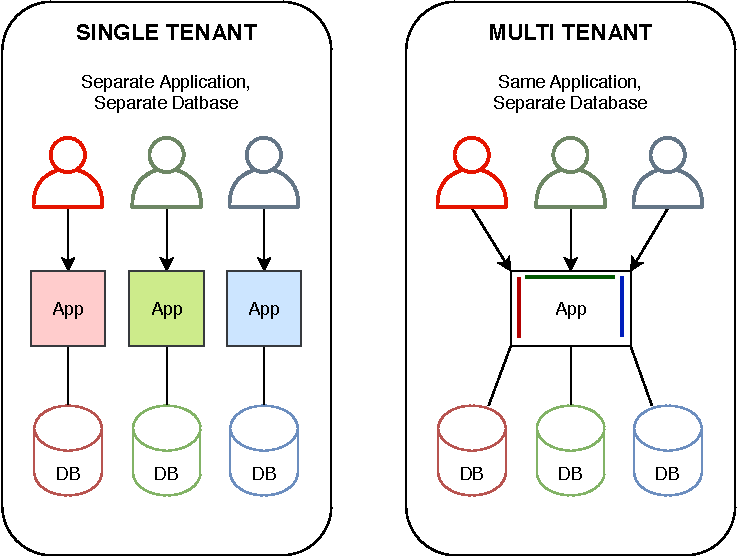
\includegraphics[width=0.94\textwidth]{images/02_3_multitenancy.pdf}
    \caption{Single Tenant vs. Multi Tenant}
    \label{fig:multitenancy}
\end{figure}

\subsection{Backend Overview}
Ad oggi non è presente un elemento definibile come \emph{layer di API} nell’applicazione. Il sistema è composto da un unico monolite che tra le tante mansioni che ha espone anche le `API'. Nello stesso sistema viene effettuato ogni genere di controllo per quanto rigurarda l'autenticazione e i parametri passati nelle richieste. Il backend è interamente scritto in PHP e si appoggia ad un database MySQL. Nonostante con gli ultimi aggiornamenti PHP offra la possibilità di programmare a oggetti, questo non è il caso del sistema preso in analisi. Per la creazione di dati che in altri linguaggi sarebbero rappresentabili attraverso oggetti, il backend utilizza un sistema di liste con elementi di tipo chiave-valore.

\subsection{Chiamate delle API}
Le chiamate dal frontend alle API intercettano il click sul documento, andando a cercare il componente su cui è stata registrata l'interazione. Tutte le richieste inviate al backend sono richieste GET HTTP. Quindi, passando un qualsiasi parametro o effettuando operazioni di aggiunta o modifica di dati, i parametri vengono aggiunti all'url, e mostrati in chiaro. Questo scelta è stata adottata anche per i metodi di registrazione e autenticazione, i più delicati dal punto di vita della sicurezza. Con la sintassi \texttt{\$\_GET} in PHP si fa riferimento a una variabile globale che contiene i parametri in GET della richiesta HTTP.
\begin{figure}[H]
\begin{alltt}
    \centering
    http://domain.it/index.php/api/v1/login?
    \centering
    _apikey=1&
    email=mariarossi2020%40studenti.unipr.it&
    password=Password123!
    callback=jQuery22404905003978295608_1605812447764&
    _=1605812447767
\end{alltt}
\caption{Esempio di richiesta GET in HTTP}
\label{fig:getlogin}
\end{figure}
Prendendo in analisi la richiesta di login in figura [\ref{fig:getlogin}], nell'url sono presenti i parametri \textsl{email} e \textsl{password} utilizzati per autenticare l'utente. Questi dati sensibili \textit{non dovrebbero appartenere all'url} dove sono visibili, ma andrebbero passati nel \emph{body} di una richiesta. Con la variabile \texttt{\$\_GET} in PHP è dunque possibile accedere anche a questi parametri.

\subsubsection{Scenario}
Il sistema, per capire quale API è stata chiamata, ricerca il metodo della richiesta passando il parametro \texttt{\$\_GET} all'interno di un costrutto condizionale di grandi dimensioni e verificando ogni chiamata possibile. In figura [\ref{fig:apicall}] viene presentata una ricostruzione di parte del codice a cui si fa riferimento. Quando il valore del parametro corrisponde al nome del metodo chiamato, nello stesso ciclo richiama l'operazione richiesta. Risulta facile notare che il codice, implementato in questo modo, presenta diversi lati negativi. Vengono ripetute parti di codice, i parametri vengono istanziati dentro ciascun \emph{if statement} e passati ai metodi che ne richiedono l'utilizzo: tutto questo all'interno della stessa condizione. Infine, i risultati di ciascuna chiamata vengono istanziati all'interno di array.
\usemintedstyle{pastie}
\begin{figure}
    \inputminted[firstline=2, lastline=15]{octave}{src/examples/old_api_call.php}
    \caption{Struttura delle chiamate Api}
    \label{fig:apicall}
\end{figure}

\subsection{Same Origin Policy}
Un'origine è definita da un \textit{protocollo}, un \textit{dominio} e una \textit{porta} di un URL. Più in generale, i documenti appartenenti a pagine web differenti sono isolati gli uni dagli altri. L'intento di questa politica è quello di consentire l'accesso a siti non sicuri, ma senza che quest'ultimi abbiano la possibilià di interferire con la sessione di chi naviga su un sito sicuro. \cite{w3c:sop}

\paragraph{I controlli} di origine vengono applicati dal browser in ogni caso di potenziale interazione tra elementi di origini diverse. Questo include, ma non è limitato a:
\begin{itemize}
    \item Codice JavaScript e Document Object Model (DOM)
    \item Cookies
    \item Chiamate AJAX (XmlHTTPRequest)
\end{itemize}

\subsubsection{Chiamate AJAX}
L'\emph{Asynchronous JavaScript and XML} è ad oggi la tecnica più utilizzata per sviluppare applicazioni web interattive. Il concetto che sta alla base di una chiamata AJAX è quello di \textit{poter scambiare dati tra client e server senza ricaricare la pagina}: lo scambio avviene in background tramite una chiamata asincrona dei dati di solito utilizzando l’oggetto \textsl{XMLHttpRequest}. Il framework \textbf{JQuery} semplifica notevolmente l'implementazione di chiamate di questo tipo, e a ciò deve la sua fama.

\subsubsection{Cross Origin Resource Sharing - CORS}
In alcuni casi, lavorare con domini differenti che interagiscono tra loro può rivelarsi \textit{una necessità}. Quando ciò accade, \textit{è possibile allentare la Same Origin Policy} in modo che non ostacoli le funzionalità di interazione tra domini dell’applicazione web. Ciò può essere fatto in diversi modi, ad esempio: dichiarando l'origine utilizzando JavaScript, l'intestazione di una chiamata, o stabilendo un sistema di autenticazione tra le due parti. Questa procedura prende il nome di \textit{Cross-Origin Resource Sharing}. L'utilizzo di questo meccanismo fa a caso nostro per quanto riguarda le chiamate delle API di Zerocoda, le quali si trovano su un dominio differente rispetto a quello della pagina web. Siccome durante il primo sviluppo dell'applicazione non si aveva pensato ad una soluzione simile, durante la nuova fase di analisi si è tenuto conto di questo aspetto. Nell'implementazione si lavorerà dunque alla stesura di API su un differente dominio, garantendone l'accesso e dichiarando affidabili le origini necessarie. Alla nascita di Zerocoda si è elaborato un modo per aggirare questo problema, piuttosto che eliminarlo alla radice.

\subsubsection{JSONP}
JSONP è l’acronimo di \emph{JSON with Padding} ed è la tecnica utilizzata per ovviare alla limitazione imposta dalla Same Origin Policy. Il suo funzionamento di base è semplice: permette a un browser di accedere a risorse remote mediante codice JavaScript, indipendentemente dall’host di origine. La tecnica permette di invocare una \textit{funzione di callback} automatizzata (come spesso viene fatto per le richieste AJAX basate su XmlHttpRequest) al ricevimento di dati. Il JSON è definito all'interno di questa funzione. Al caricamento del file JavaScript, l'interprete esegue la funzione di callback, che è così in grado di restituire il JSON al client.
\usemintedstyle{friendly}
\begin{figure}[H]
    \inputminted{octave}{src/examples/jsonp.js}
    \caption{JSONP Callback - Login}
    \label{fig:jsonpexample}
\end{figure}
Nella figura [\ref{fig:jsonpexample}] viene presentata la callback utilizzata per restituire all'utente i propri dati dopo un'autenticazione andata a buon fine. La chiamata AJAX (invocata da JQuery) viene così mascherata con il caricamento di un file JavaScript. La stringa di numeri presente sul parametro callback viene inizializzata con un valore corrispondente al nome randomico di una funzione appena creata da uno script server-side. Come si osserva dalla precedente figura [\ref{fig:getlogin}] il server ha conoscenza della funzione da andare a creare, in quanto ottiene questa informazione dai parametri del metodo GET utilizzato. Il codice JavaScript inserito nella pagina HTML utilizza poi questa funzione per passare i parametri che normalmente vengono restituiti con un file JSON. Si tratta sostanzialmente di un'invocazione di funzione.

%%%%%%%%%%%%%%%%%%%%%%%%%%%%%%%%%%%%%%%%%%%%%%%%%%%%%%%%%%%%%%%%%%%%%%%%%
\section{Architettura Odierna}
Nell'immagine [\ref{fig:oldarchitecture}] viene rappresenta l'architettura \emph{attuale} del sistema. Di seguito vengono analizzate le tecnologie che utilizza.
\begin{figure}[H]
    \centering
    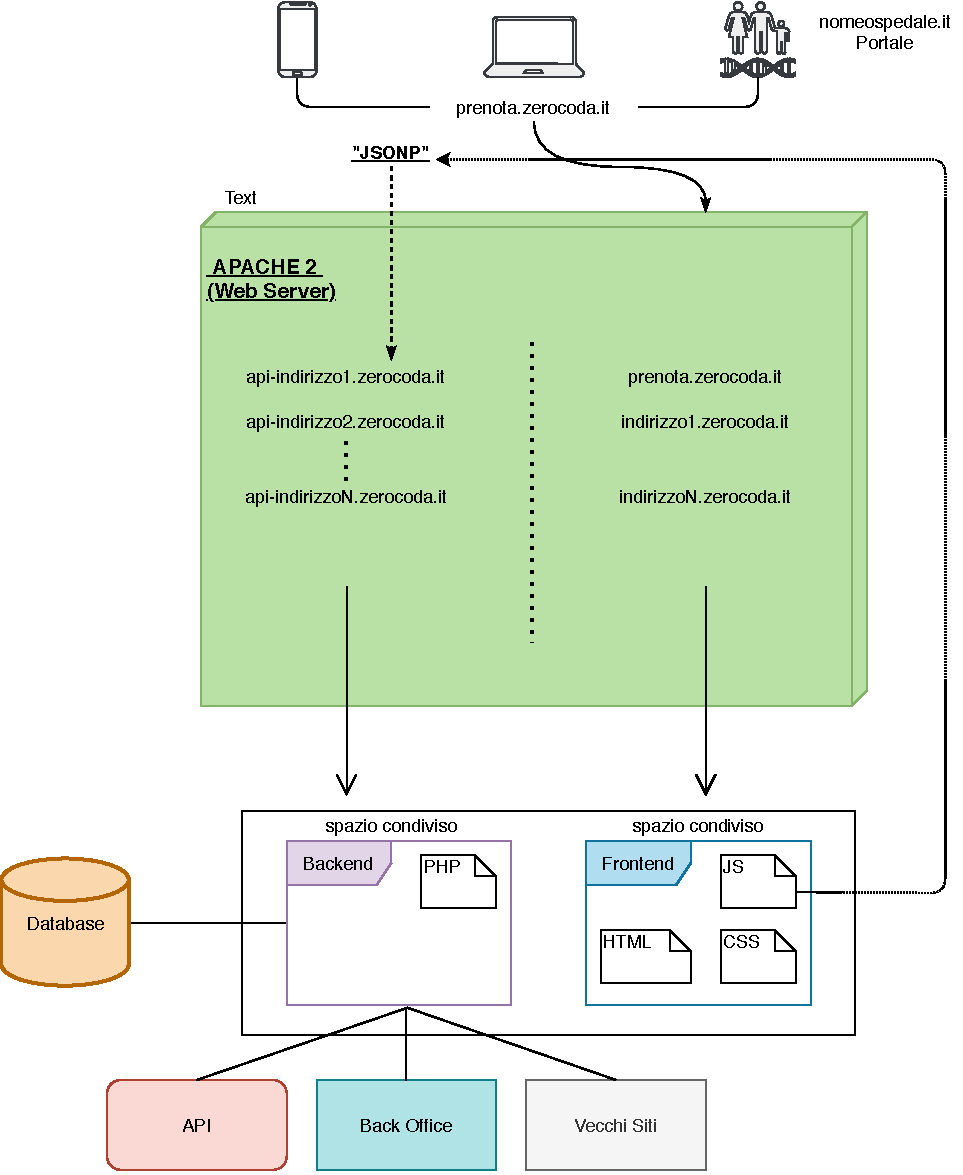
\includegraphics[width=0.95\textwidth]{images/02_4_old_architecture.pdf}
    \caption{Architettura del Sistema di Partenza}
    \label{fig:oldarchitecture}
\end{figure}

\subsection{Web Server Apache}
A livello di file system si ha uno spazio condiviso per il backend (interamente in PHP) e uno spazio condiviso per il frontend, contenente i soli contenuti statici (HTML, CSS e immagini). Il backend funge da colonna portante per diversi componenti:
\begin{itemize}
    \item \textbf{backoffice}: sostanzialmente l'interfaccia amministrativa di Zerocoda. Attraverso questa interfaccia è possibile gestire tutto il sistema. Viene utilizzata principalmente per aggiungere quelli che si definiscono 'slot', ma può essere anche utilizzata per creare e gestire utenti. Uno \emph{slot} è un posto prenotabile per un servizio in un determinato giorno e in una determinata fascia oraria. Con il backoffice un amministratore può aggiungere in modo semi-automatico gli slot per un determinato servizio, scegliendone il numero per ogni ora e lo stato (abilitato o disabilitato) al momento della creazione.
    \item \textbf{vecchi siti } precedenti al refactoring. Prima di questo refactoring il frontend del sito era stato aggiornato. Nulla è stato cambiato per quanto riguarda il funzionamento, solo gli elementi grafici sono stati modificati per rispondere ad uno stile più moderno. Nonostante ciò, si è scelto di mantenere online il frontend per alcuni siti, che in questo modo rimane sempre a carico di Apache.
    \item \textbf{API}: le chiamate esposte in precedenza: il vero target dell'elaborato. Le Api a cui si fa riferimento quando si invia una richiesta per effettuare un'operazione sono le stesse per tutti i dispositivi. Non c'è differenza che si acceda da un browser web, un dispositivo mobile, o dal portale di un sito con configurazione personalizzata.
\end{itemize}   
Con le caratteristiche attuali Apache2 funziona esclusivamente da Web Server.

\subsection{Virtual Hosting}
Non tutti i siti hanno abbastanza traffico da giustificare il costo di un web server dedicato, pertanto la loro condivisione su un singolo web server può essere una buona soluzione per abbassarne il costo. Il \emph{virtual hosting} viene incontro a questa esigenza, permettendo ad un unico server web di “ospitare” più siti (e/o applicazioni) web, i quali condivideranno, secondo opportune politiche di gestione, le risorse di elaborazione del server stesso. Consolidare più servizi su un’unica macchina è una pratica comunemente adottata poiché permette di ottimizzare l’utilizzo delle risorse hardware disponibili. Senza il virtual hosting, si renderebbe necessario attivare una nuova macchina server per ogni nuovo sito o applicazione web, con un conseguente aumento dei costi ed un possibile sottoutilizzo delle risorse hardware. Con l'attuale architettura \textit{Apache ospita al suo interno una serie di virtual host}.

\paragraph{Funzionamento} Il server Apache, con un unico indirizzo IP, ospita più di un nome di dominio. I diversi domini, com'è  possibile osservare dalla figura [\ref{fig:virtualhosting}] condividono la stessa porta, ma si può anche assegnare a ciascun dominio una porta specifica.

\begin{figure}[H]
    \centering
    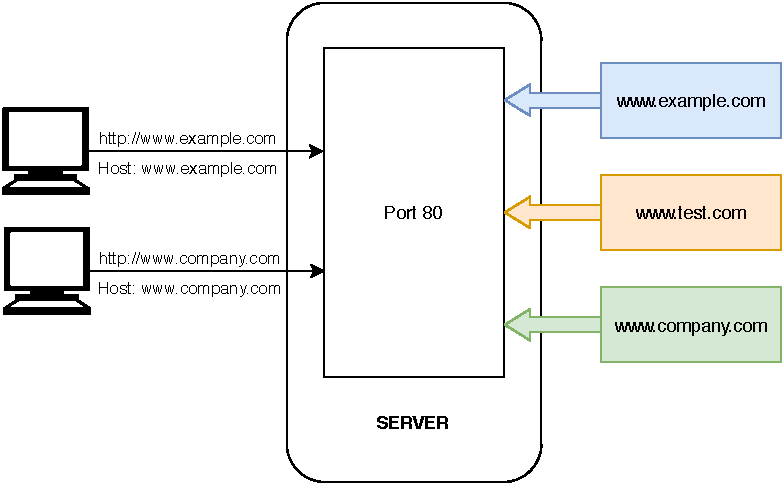
\includegraphics[width=0.95\textwidth]{images/02_5_virtual_hosting.pdf}
    \caption{Funzionamento del Virtual Hosting}
    \label{fig:virtualhosting}
\end{figure}

\subsection{Database MySQL}
Il dialogo con il database avviene attraverso il codice PHP del backend. È compito del server Apache fornirne l'accesso per una serie di indirizzi (le API). Il database è \textit{unico per tutti gli enti Zerocoda}, anche gli enti `premium' interrogano la stessa base di dati degli altri. Coloro che hanno richiesto un metodo di accesso diverso da quello standard si limitano ad avere una tabella isolata dagli altri, contenente i dati dei propri utenti. Poiché questa tipologia di enti ha gli utenti su una tabella diversa, avrà anche API apposite per interrogarla. Questa API si trova sempre all'interno dello stesso backend, insieme alle altre.

%%%%%%%%%%%%%%%%%%%%%%%%%%%%%%%%%%%%%%%%%%%%%%%%%%%%%%%%%%%%%%%%%%%%%%%%%
\section{Limiti del Database}
La struttura del database non corrisponde a quella che ci si aspetterebbe in un tipico sistema di prenotazioni utente. Nel database sono infatti contenute diverse tabelle di configurazione per il software, per lo più utilizzate nel backoffice in fase di amministrazione. Queste tabelle contengono ad esempio i giorni festivi all 'interno di un anno (in cui non è quindi possibile prenotare determinati servizi), o i giorni della settimana per evitare prenotazioni errate nei weekend dove alcune strutture possono essere chiuse. Tra queste sono presenti anche tabelle per la configurazione dei campi utente in fase di registrazione e altre contenti i messaggi di errore da restituire. Questi tipi di tabelle vengono utilizzate quindi come metodo di controllo nelle query. Inoltre, sul database vengono salvati anche i log riguardanti il funzionamento dello stesso: è logico dedurre che, in caso di malfunzionamento, non c'è modo di verificare questi documenti.

\subsection{Autenticazione}
 Per autenticarsi l'utente fornisce la propria email e la propria password, che, al momento del primo accesso, contribuiscono alla generazione di un token casuale da parte del sistema. Per gli accessi successivi questo stesso token viene utilizzato per identificare l'utente. In principio Zerocoda era sprovvista di un sistema di autenticazione mediante token randomici. Questa funzionalità è stata introdotta poco prima del refactoring, tuttavia i token di autenticazione vengono salvati sul database e interrogati dallo stesso backend piuttosto che da un server esterno. Nella progettazione della nuova architettura si è pensato a questo problema, gestendolo attraverso un apposito microservizio.

\subsection{Verifica delle API Keys}
Non è presente nessuna struttura intermediaria tra client e server che si occupi di fare i controlli necessari per la verifica delle api keys, pertanto queste operazioni si traducono in delle semplici query alla base di dati. L'Api Key deve essere un \emph{campo obbligatorio} nella richiesta di un'operazione. Questa permette di identificare l'ente/i corrispondenti, mostrandone i relativi dati sulla pagina. Ad esempio, un utente che accede a Zerocoda deve essere in grado di vedere i soli enti e servizi corrispondenti ad un'api key, mentre accedendo ad un portale di un sito con una propria configurazione deve vedere i soli dati relativi a prenotazioni e servizi di quella struttura. Anche il controllo dell'Api Key, come per l'autenticazione, si è deciso di delegarlo a un nodo intermedio.

\subsection{Ridondanza dei Dati}
Come le precedenti, anche la ridondanza dei dati è un limite che ha dato diversi problemi durante la manutenzione del software. Il database presenta due tabelle con lo stesso scopo: \textit{users} e \textit{bookers}. Inizialmente le due erano state pensate con compiti diversi. La prima avrebbe registrato i dati degli \emph{amministratori di sistema}, coloro che hanno necessità di accedere al backoffice, mentre la seconda avrebbe contenuto i dati degli \emph{utenti finali} di Zerocoda. La continua manutenzione degli ultimi anni ha portato il software ad essere sviluppato sempre da \textit{persone diverse}. Questo, unito all'ambiguo nome dato a tabelle, ha portato i dati ad essere incosistenti da quelli pensati nel disegno orginale. Al momento, i dati di un utente in fase di registrazione vengono quindi salvati su due tabelle distinte.

\subsection{Vincoli di Integrità}
I vincoli di integrità permettono alle tabelle di disporre di \emph{regole rigide} riguardanti i dati che è possibile inserire al loro interno. Il database non le utilizza in tutte le tabelle. Il modo in cui i dati vengono inseriti o eliminati dal database deve essere sempre lo stesso e coerente negli anni. Non essendo così, anche i metodi di interrogazione ne risentono. Un sistema di questo tipo dovrebbe avere poche query, semplici e comprensibili, tuttavia la disuguaglianza di alcuni valori all'interno del database non lo rende possibile. Alcune prenotazioni, eliminate da utenti o amministratori, presentano valori \emph{null}, mentre altre hanno il valore `0' che le identifica come `non prenotate'. Quando è necessario eliminare un dato presente su più tabelle, spesso occorre fare più di una query, controllandone il risultato. Questi problemi si sarebbero potuti evitare in fase di progettazione.
%%%%%%%%%%%%%%%%%%%%%%%%%%%%%%%%%%%%%%%%%%%%%%%%%%%%%%%%%%%%%%%%%%%%%%%%%
In questo capito è illustrato il funzionamento attuale del sistema e le tecnologie che utilizza, con cenni riguardenti le soluzioni pensate per ogni specifico problema. Vengono presentate l'architettura del sistema di partenza e quella di arrivo, in riferimento al modello di sviluppo dell'\emph{ingegneria del software} seguito.

\section{Reverse Enginering}
\newtheorem*{def:reverseengineering}{Definizione}
\begin{def:reverseengineering}
    La reingegnerizzazione è quel processo di esame, analisi e alterazione di un sistema software esistente, col fine di ricostruirlo in una nuova forma, e la successiva implementazione. \cite{chikofsky:reverseengineering} Nel processo di reingegnerizzazione è compresa anche la riprogettazione del software, mentre quando si parla di reverse engineering si fa riferimento all'analisi.
\end{def:reverseengineering}
Il reverse engineering del codice permette di invertire i processi di sviluppo e produzione di un software e quindi di ottenere uno sguardo prezioso dietro le quinte di un programma. Attraverso lo studio dettagliato del codice sorgente è possibile comprendere, riscrivere o ricostruire l’architettura di un programma, il suo funzionamento e le sue strutture interne. Apparentemente la reingegnerizzazione non dovrebbe essere fatta per modificare i requisiti funzionali del sistema. In realtà, spesso quando si applica questa tecnica ci si accorge, in fase di riprogettazione, che alcuni requisiti, dopo anni di sviluppo, non sono più validi e andrebbero tolti dal disegno, mentre altri, nuovi, andrebbero introdotti.

\subsection{I motivi}
La pandemia di quest'ultimo anno ha portato l'azione di refactoring su \emph{Zerocoda} ad essere a tutti gli effetti una necessità. Il distanziamento sociale è un bisogno per ogni tipo servizio offerto ad una clientela più o meno vasta, e tenere traccia dei clienti e del loro numero temporizzando gli accessi al servizio è senza alcun dubbio la soluzione migliore. Nello stato attuale, tuttavia, l'applicazione non rispetta i requisiti funzionali per essere rilasciata ad un pubblico di tipo \emph{enterprise}. Sono sempre di più le aziende che hanno richiesto l'inserimento dei loro servizi nell'applicazione. L'inserimento di nuovi servizi porterebbe all'aumento delle richieste da parte dei client, più richieste a più dati da elaborare, e più dati a un sovraccarico. L'applicazione non è pronta a uno scenario di questo tipo, pertanto urge un refactoring mirato all'introduzione di nuove tecnologie, che renda il software più scalabile in prevenzione del nuovo numero di clienti sulla piattaforma.

Questo rappresenta il motivo principale, quello che ha portato l'azione di refactoring, dapprima solo ipotizzata da coloro che già lavoravano al sistema, a un inizio di progettazione. Normalmente le esigenze possono essere anche altre:

\begin{itemize}
    \item il team di sviluppo è cambiato e sono subentrati altri programmatori che non hanno conoscenze in merito al sistema;
    \item la documentazione è assente del tutto o, se presente, dopo anni di sviluppo e modifiche non è stata aggiornata e risulta obsoleta;
    \item  l'introduzione di piccoli cambiamenti risulta complessa e costosa da affrontare in termini di tempo e risorse;
    \item il software è spesso soggetto a continue correzioni di bug, indice che la struttura è precaria e mal progettata;
    \item numerose correzioni sono state apportare e si è verificato il fenomeno ``architectural drift'' (deriva architetturale), cioè il sistema si è spostato molto dal disegno originale che non è più chiaro
    \item i metodi e gli strumenti di sviluppo originali sono ormai superati ed è difficile trovare programmatori con queste conoscenze.
\end{itemize}

%%%%%%%%%%%%%%%%%%%%%%%%%%%%%%%%%%%%%%%%%%%%%%%%%%%%%%%%%%%%%%%%%%%%%%%%%
\section{Modello di Sviluppo}
Come \textit{metodologia di sviluppo} si è scelto di adottarne una di tipo \textbf{agile}. Secondo questo \emph{principio teorico}, il punto di partenza è costituito dalla specifica dei requisiti, mentre lo sviluppo vero e proprio del software avviene solo in seguito.

\subsection{Waterfall Model}
Il modello a cascata è un \textbf{ciclo di vita lineare}, che suddivide il processo di sviluppo in fasi di progetto consecutive. A differenza dei modelli iterativi, \textit{ogni fase viene eseguita solo una volta}. Con questo modello il progetto viene organizzato in una sequenza di fasi, ciascuna delle quali produce un output che costituisce l’input per la fase successiva.

\subsubsection{Origini}
Lo sviluppo del modello viene attribuito allo scienziato informatico Winston W. Royce, che tuttavia, non è stato il suo vero inventore. Al contrario, il suo articolo pubblicato nel 1970 “Managing the Development of Large Software Systems” \cite{royce:softwaredevelopment} conteneva una critica aperta nei confronti dei cicli di vita lineari. Come alternativa, presentava un modello iterativo-incrementale, in cui ogni fase attinge a quella precedente e ne verifica i risultati. 

\paragraph{Il modello di Royce} è cosituito da sette fasi eseguite in diversi passaggi (iterazioni):

\begin{enumerate}
    \item Requisiti di sistema
    \item Requisiti di software
    \item Analisi
    \item Progettazione
    \item Implementazione
    \item Test
    \item Esecuzione e Manutenzione
\end{enumerate}
Il modello a cascata si ispira alle fasi definite da Royce, ma prevede solo un’iterazione.

\subsubsection{Funzionamento}
Nella pratica vengono utilizzate diverse versioni del modello a cascata. Attualmente sono in uso modelli che suddividono i processi di sviluppo in cinque fasi. Le fasi 1, 2 e 3, definite da Royce, sono riunite in un’unica fase di progetto, chiamata analisi dei requisiti. [\ref{fig:waterfallmodel}]
\begin{enumerate}
    \item Analisi: pianificazione, analisi e specificazione dei requisiti
    \item Progettazione: progettazione e specificazione del sistema
    \item Implementazione: programmazione e test di modulo
    \item Test: integrazione di sistema, test di sistema e test di integrazione
    \item Esecuzione: rilascio, manutenzione, miglioramento
\end{enumerate}
\begin{figure}[H]
    \centering
    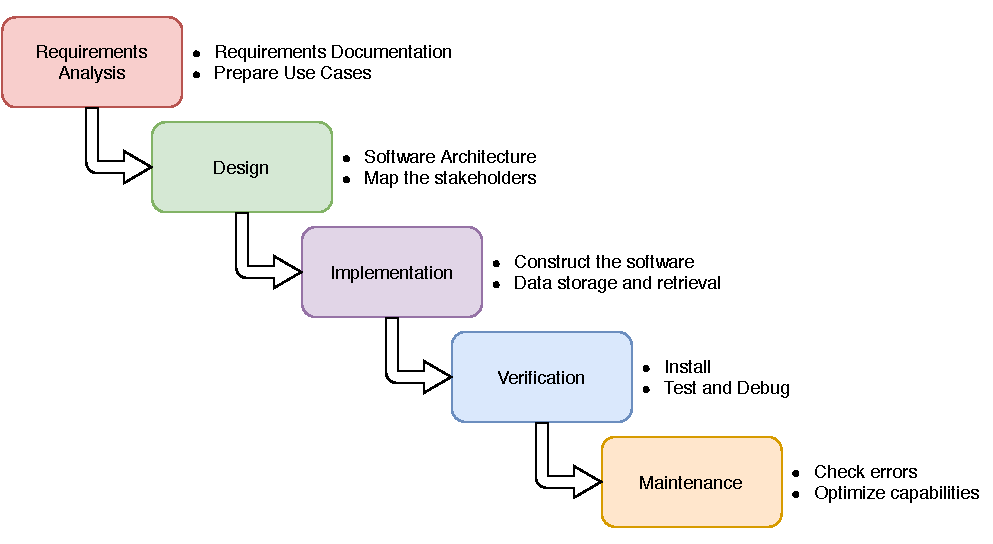
\includegraphics[width=0.94\textwidth]{images/02_1_waterfall_model.pdf}
    \caption{Fasi del Modello a Cascata}
    \label{fig:waterfallmodel}
\end{figure}
Il modello da noi utilizzato rappresenta un'\textit{estensione del modello a cascata}, in quanto l'eseguire ogni fase una sola volta comporta un grande vincolo. Ad ogni fase infatti si confrontano e verificano i risultati ottenuti con quelli della fase precedente. Partendo da un'analisi delle esigenze richieste dall'applicazione, dai suoi limiti e dalle necessità dei clienti, si è poi passati all'individuazione di una strada per lo sviluppo.

%%%%%%%%%%%%%%%%%%%%%%%%%%%%%%%%%%%%%%%%%%%%%%%%%%%%%%%%%%%%%%%%%%%%%%%%%
\section{Nuova Architettura}
\begin{figure}[H]
    \centering
    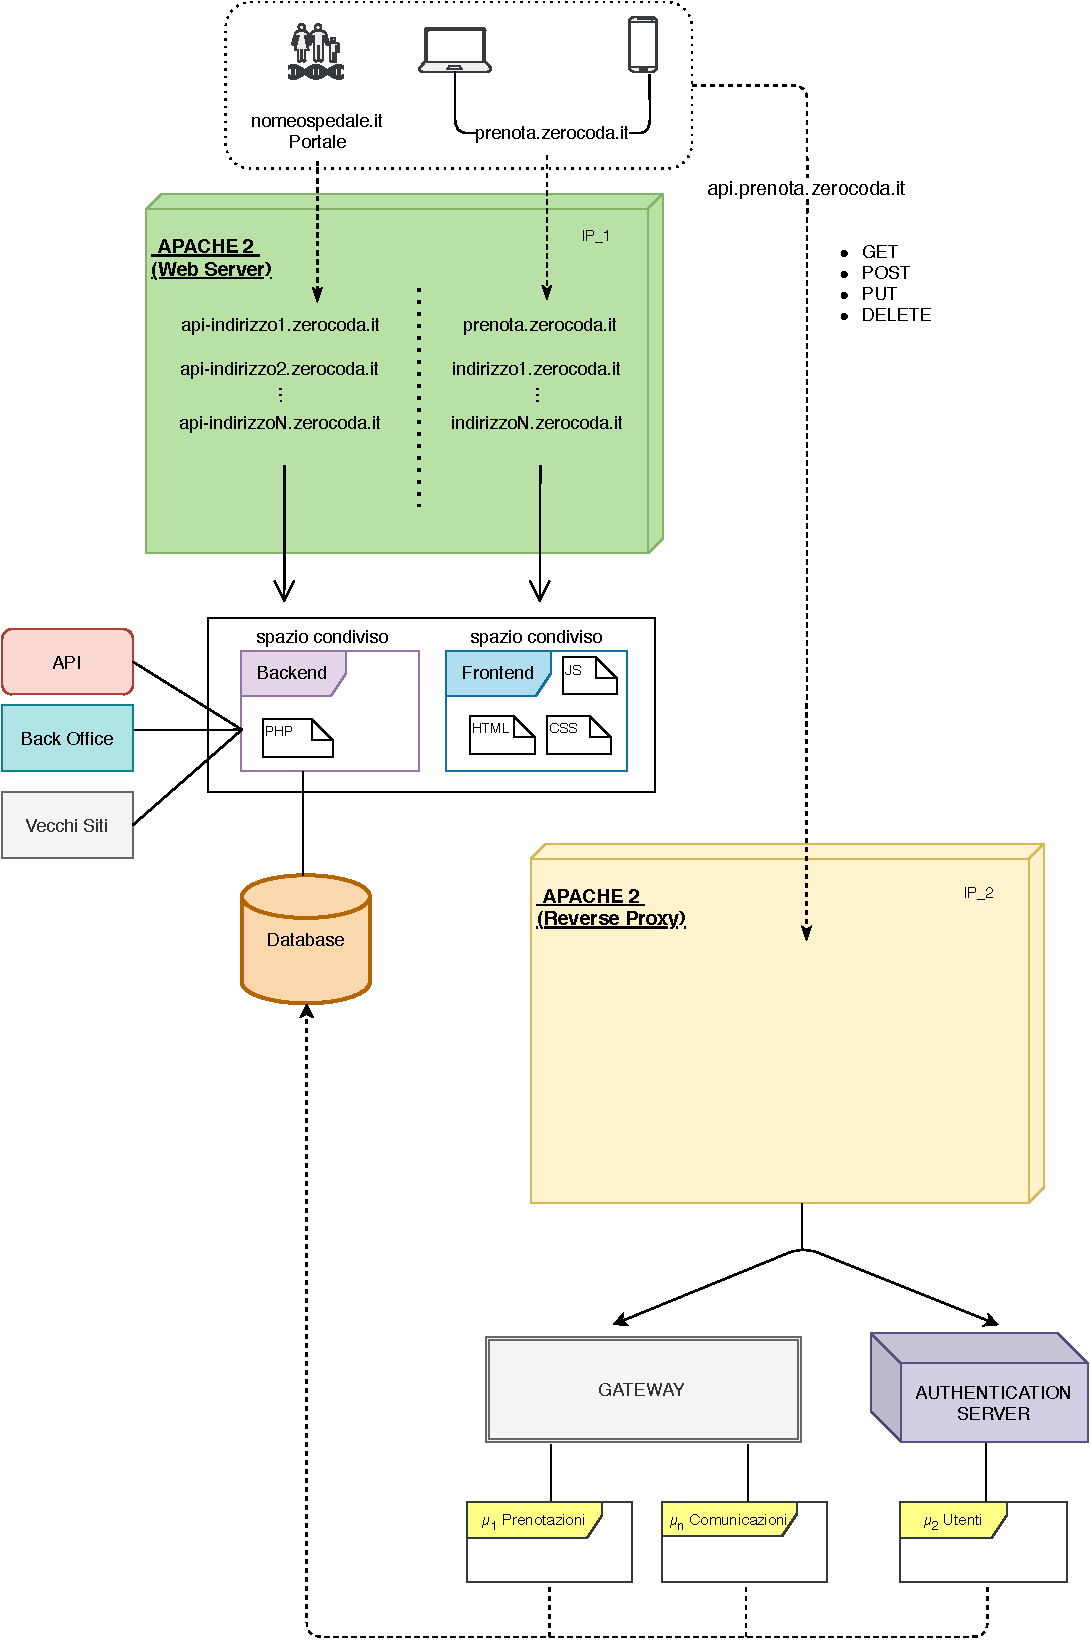
\includegraphics[width=0.84\textwidth]{images/02_11_new_architecture.pdf}
    \caption{Architettura del Sistema di Arrivo}
    \label{fig:newarchitecture}
\end{figure}

\subsection{Monolite}
%Come si vede in figura [\ref{fig:newarchitecture}] parte della nuova architettura comprende una parte rimasta inviariata dalla precedente: il Monolite. Prendiamo ad esempio un ospedale che ha configurato un portale per la prenotazione sul proprio sito: \emph{www.hospital.com}. Questo ospedale, richiedendo il livello di personalizzazione più alto per la propria utenza, ha richiesto anche una api apposita per gestirne le operazioni, che prende il nome di \emph{api-hospital.zerocoda.it}. La motivazione che porta il monolite a continuare ad esistere in questa prima fase di refactoring è che questa API risiede sul server Apache di partenza.
Come si vede in figura [\ref{fig:newarchitecture}] parte della nuova architettura comprende un componente rimasto invariato dall'architettura precedente: il Monolite. Questo infatti, per una prima fase del processo evolutivo, servirà ancora le vecchie API al backoffice. Il monolite verrà meno dall'architettura solo quando comincerà la fase di refactoring inerente al database. Con essa, verrà rifatto il backoffice e le API implementate saranno riadattate con le nuove query. A questo punto anche il backend verrà rimosso, permettendo all'applicazione di utilizzare il Web Server solo per ottenere il frontend.

\subsection{Scenario}
Quando l'utente si connette al sito \emph{www.prenota.zerocoda.it} viene fatta la risoluzione del DNS e il reindirizzamento sul \textit{vecchio server}. Questo rimane identico al precedente e comprende sempre frontend, backend e database. Durante il caricamento della pagina all'utente vengono sempre restituiti i componenti statici e il JavaScript, aggiornato per utilizzare le nuove API. Quando si deve fare un'operazione si utilizza ora un nuovo indirizzo \emph{api.prenota.zerocoda.it}. L'indirizzo consente le invocazioni di metodi REST, appoggiandosi a un server Apache con un indirizzo IP diverso dal precedente. Quest'ultimo funziona da Reverse Proxy, limitandosi a inoltrare le richieste ad una serie di microservizi. Ciascun microservizio interroga la stessa base di dati, che rimane invariata. Prima anche un ente che avesse richiesto una configurazione con un portale Zerocoda sul proprio sito sarebbe dovuto passare per il Web Server principale. Con l'introduzione delle nuove API sarà possibile utilizzare l'indirizzo fornito, che consente di passare direttamente per il Reverse Proxy.

%%%%%%%%%%%%%%%%%%%%%%%%%%%%%%%%%%%%%%%%%%%%%%%%%%%%%%%%%%%%%%%%%%%%%%%%%